\chapter{Architecture of lightweight Threads in Java}

\section{Continuation}

A continuation is a sequence of instructions, that can be yielded and continued. The following example shows how a continuation can calculate the sum of the first five natural numbers while yielding after each increment.

\begin{lstlisting}[language=custom-java]
    var scope = new ContinuationScope("ContinuationScope");
    var continuation = new Continuation(scope, () ->  {
        int n = 0;
        for(int i = 0; i < 6; i++) {
            n = n + i;
            System.out.println("i: " + i + "\t" + "n: " + n);
            Continuation.yield(scope);
        }
    });

    while(!continuation.isDone()) {
        System.out.println();
        continuation.run();
    }
\end{lstlisting}

A continuation requires two arguments: A scope and a runnable. First, a scope is created. Then the continuation is created. Afterwards, the continuation is repeatedly run in a loop until it is done.
\\
\\
The scope is used to allow continuations to be nested. Each continuation has exactly one parent continuation and exactly one child continuation. Continuations run on top of kernel-level Java threads, which are referred to as carrier-threads. Every Java carrier-thread has exactly one continuation as one of its attributes. This continuation is supposed to be the innermost one.

\subsection{Stack}
Each continuation has two stacks: One for objects and one for non-objects. Project Loom calls the continuation stack horizontal stack and the thread stack vertical stack. The abbreviated versions are called h-stack and v-stack.
When a continuation yields, it will be unmounted. Unmounting copies the continuation frames from the thread stack to the continuation stack. Afterwards, the continuation frames are removed from the thread stack. Project Loom calls this process freezing.
When a continuation starts or continues, it will be mounted. Mounting is the reverse process of unmounting. Therefore project Loom calls this process thawing. \cite{OpenJDK:wiki}

\begin{figure}[h]
    \centering
    \begin{subfigure}[b]{1.0\textwidth}
        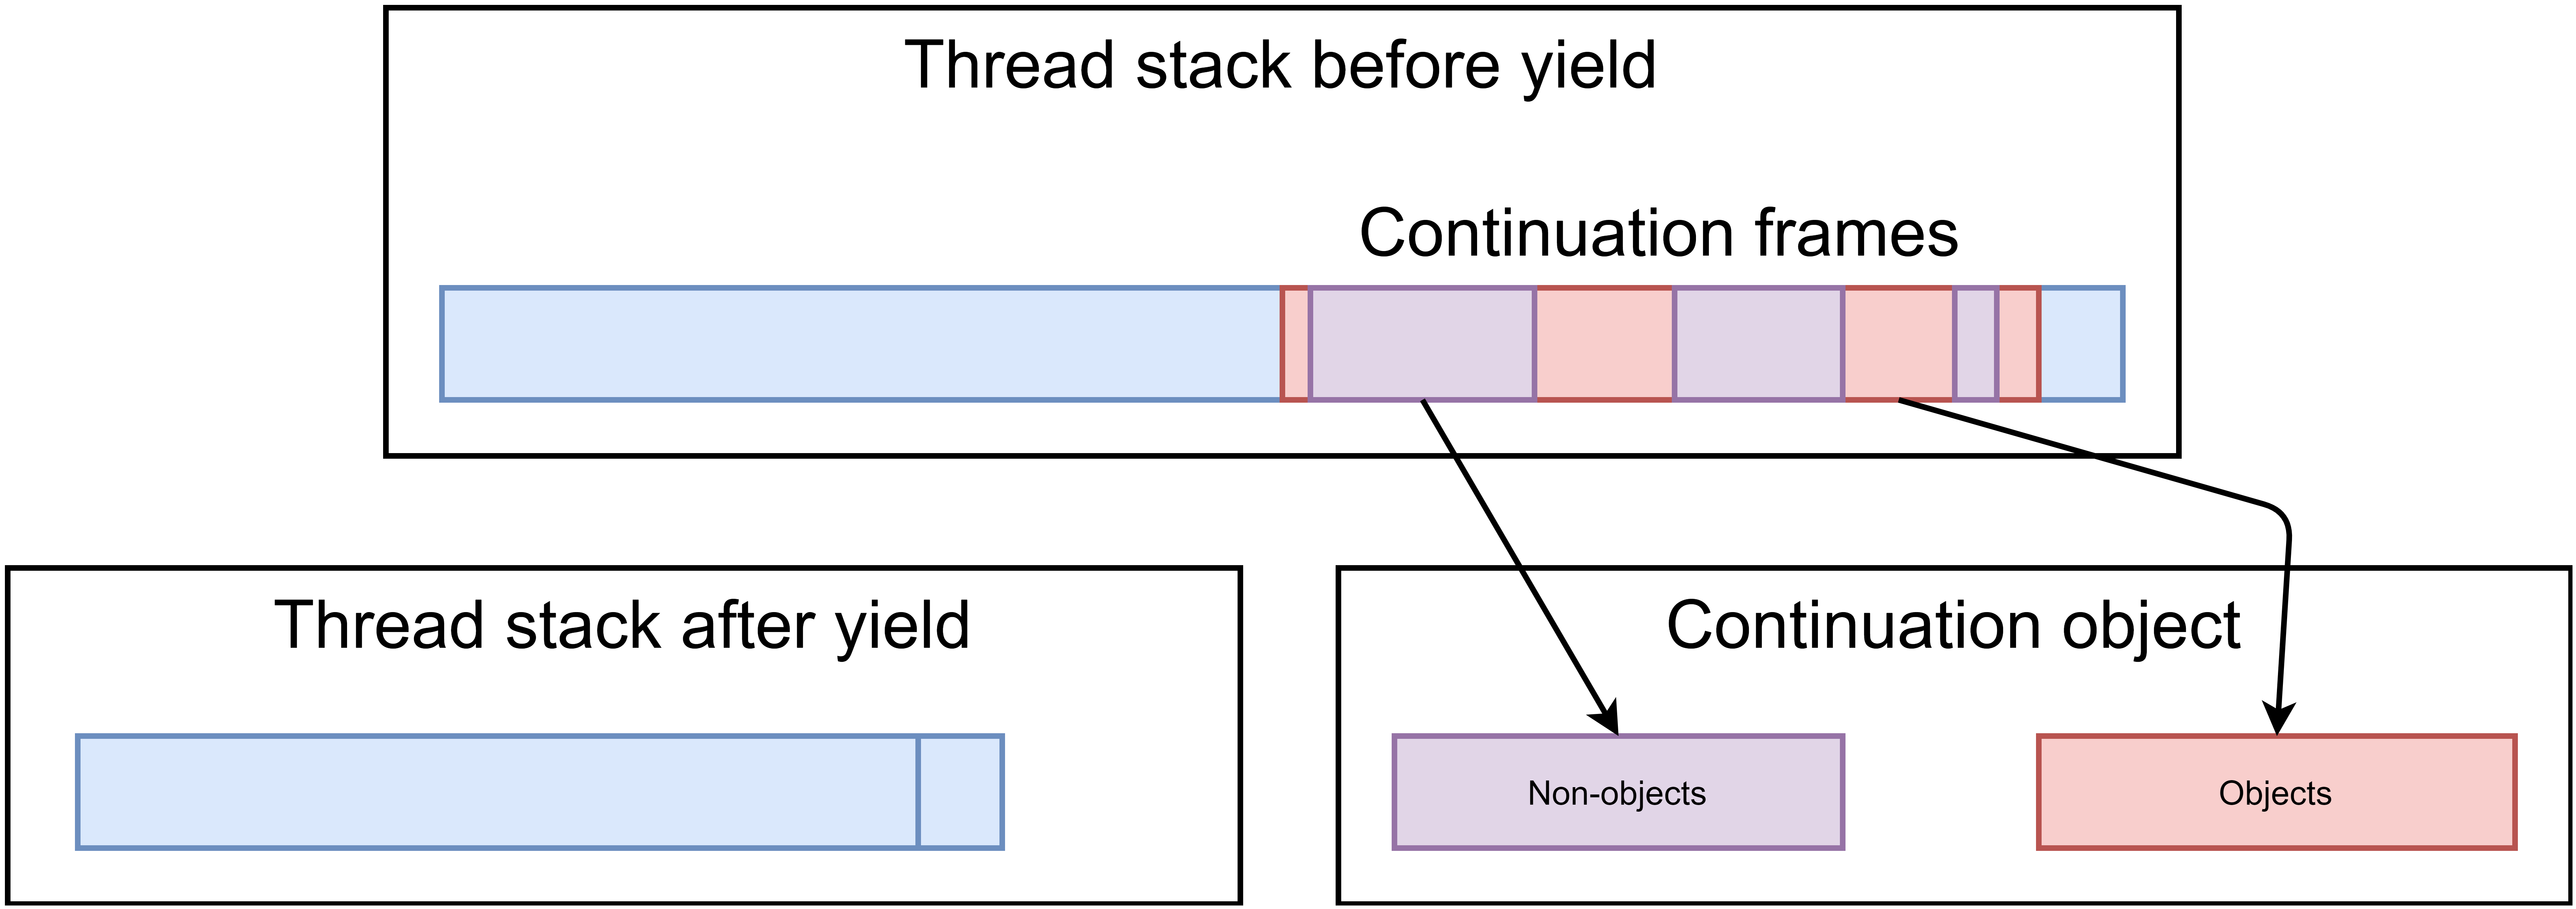
\includegraphics[width=1.0\linewidth]{img/freeze-jvmls-2019.png}
    \end{subfigure}
    \caption{Freeze \cite{OpenJDK:jvmls:2019}}
    \label{freeze}
\end{figure}

Looking at the previously mentioned two stacks on code level: One stack is an integer array for primitive values and metadata. The other one is an object array for references. All stack related methods exist twice: Once for the integer array and once for the object array. The methods are very similar. Therefore this thesis will only explain one set of them, which is the integer set.
\\
\\
Project Loom uses an integer sp as a stack pointer. Every time the stack is changed, the stack pointer will be updated. This is done by using the fixDecreasingIndexAfterResize method. As an example observe fixDecreasingIndexAfterResize using the arguments: index = 5, oldLength = 10, newLength = 20. It returns 15. The new stack pointer is therefore 15. That means that if a stack size gets changed, the remaining values are inserted starting at the end.

\begin{lstlisting}[language=custom-java]
    private int sp = -1; // index into the h-stack

    private int fixDecreasingIndexAfterResize(int index, int oldLength, int newLength) {
        return newLength - (oldLength - index);
    }
\end{lstlisting}

\myparagraph{getStack}
The getStack method is used to expand the stack. First, the program will test, whether the stack is null. If that is the case, the stack has not been created yet. Then the program will create the stack and adjust the stack pointer. If the stack is not empty, the program will create a new stack, that is big enough to fit the old and the new frames. Then it will copy the old frames into the new stack. Afterwards, the continuation's stack is set to the new stack. The stack pointer will be updated. The return value is boolean. It is True when getStack succeded. The method fails when the old stack length is larger than the new one.

\myparagraph{resizeStack}
Similar to how the getStack method expands the stack, the resizeStack method shrinks it. In contrast to the getStack method, the resizeStack method is a void and does not require to return a boolean on whether it succeeded or not.

\myparagraph{maybeShrink}
The maybeShrink method is called after yielding. It checks whether the stack size is bigger than a watermark it keeps track of. If it is, the watermark will be set to the stack size. Therefore if maybeShrink is called without adjusting the watermark, that means, that the stack size has not increased since the last time. If maybeShrink is called ten times without adjusting the watermark, the resizeStack method will be called with the watermark as it's argument.

\subsection{Critical Sections}
Project Loom solves critical sections with a classic semaphore design. The method pin increments the semaphore cs and the method unpin decrements it.

\begin{lstlisting}[language=custom-java]
    private short cs; // critical section semaphore

    public static void pin() {
        Continuation cont = currentCarrierThread().getContinuation();
        if (cont != null) {
            if (cont.cs == Short.MAX_VALUE)
                throw new IllegalStateException("Too many pins");
            cont.cs++;
        }
    }

    public static void unpin() {
        Continuation cont = currentCarrierThread().getContinuation();
        if (cont != null) {
            if (cont.cs == 0)
                throw new IllegalStateException("Not pinned");
            cont.cs--;
        }
    }
\end{lstlisting}

\subsection{Intrinsics}
Project Loom uses intrinsics to increase performance. Usually, if there is an intrinsic version of a function, there will still be a non-intrinsic one. In this case, there are no non-intrinsic versions of the functions. The following functions are exclusively intrinsic and relevant for this thesis:
\begin{lstlisting}[language=custom-java]
    @HotSpotIntrinsicCandidate
    private static long getSP()

    @HotSpotIntrinsicCandidate
    private void doContinue() 

    @HotSpotIntrinsicCandidate
    private static int doYield(int scopes)
\end{lstlisting}

For the x86 platform the following functions in stubGenerator\_x86\_64.cpp create the bytecode for the intrinsic versions of the functions named above:

\begin{lstlisting}[language=C++]
    address generate_cont_getSP()

    address generate_cont_thaw(bool return_barrier, bool exception)

    RuntimeStub *generate_cont_doYield()
\end{lstlisting}

In these functions, the maintainers of project Loom use their macroassembler. The macroassembler class can be found in src/hotspot/cpu/x86/macroAssembler\_x86.cpp. The yield method also utilizes two other big classes. One is a codebuffer located in src/hotspot/cpu/x86/asm/codeBuffer.cpp and the other is a oopmap, used for garbage collection, located in src/hotspot/share/compiler/oopMap.cpp.
\\
Analyzing these functions goes beyond the scope of this thesis.

\subsection{Run}
When a continuation gets started or continued the run method is called.
First the run method mounts the continuation. Mounting is realized using a VarHandle, which atomically sets a boolean to true.
\\
\\
Afterwards the current carrier-thread's continuation has to be updated. As an example the current carrier-thread's continuation before the update will be called bar. The new continuation will be called foo.

\begin{lstlisting}[language=custom-java]
    Thread t = currentCarrierThread();
    if (parent != null) {
        if (parent != t.getContinuation())
            throw new IllegalStateException();
    } else
        this.parent = t.getContinuation();
    t.setContinuation(this);
\end{lstlisting}

foo is not supossed to have a parent at this point of time. If foo has a parent, that parent has to be bar. If it is not, something seriously went wrong and an error is thrown. The expected outcome is, that foo has no parent. In that case foo will become the child bar. Afterwards foo will become the current carrier-threads's continuation.

\begin{figure}[H]
    \centering
    \begin{subfigure}[b]{0.45\textwidth}
        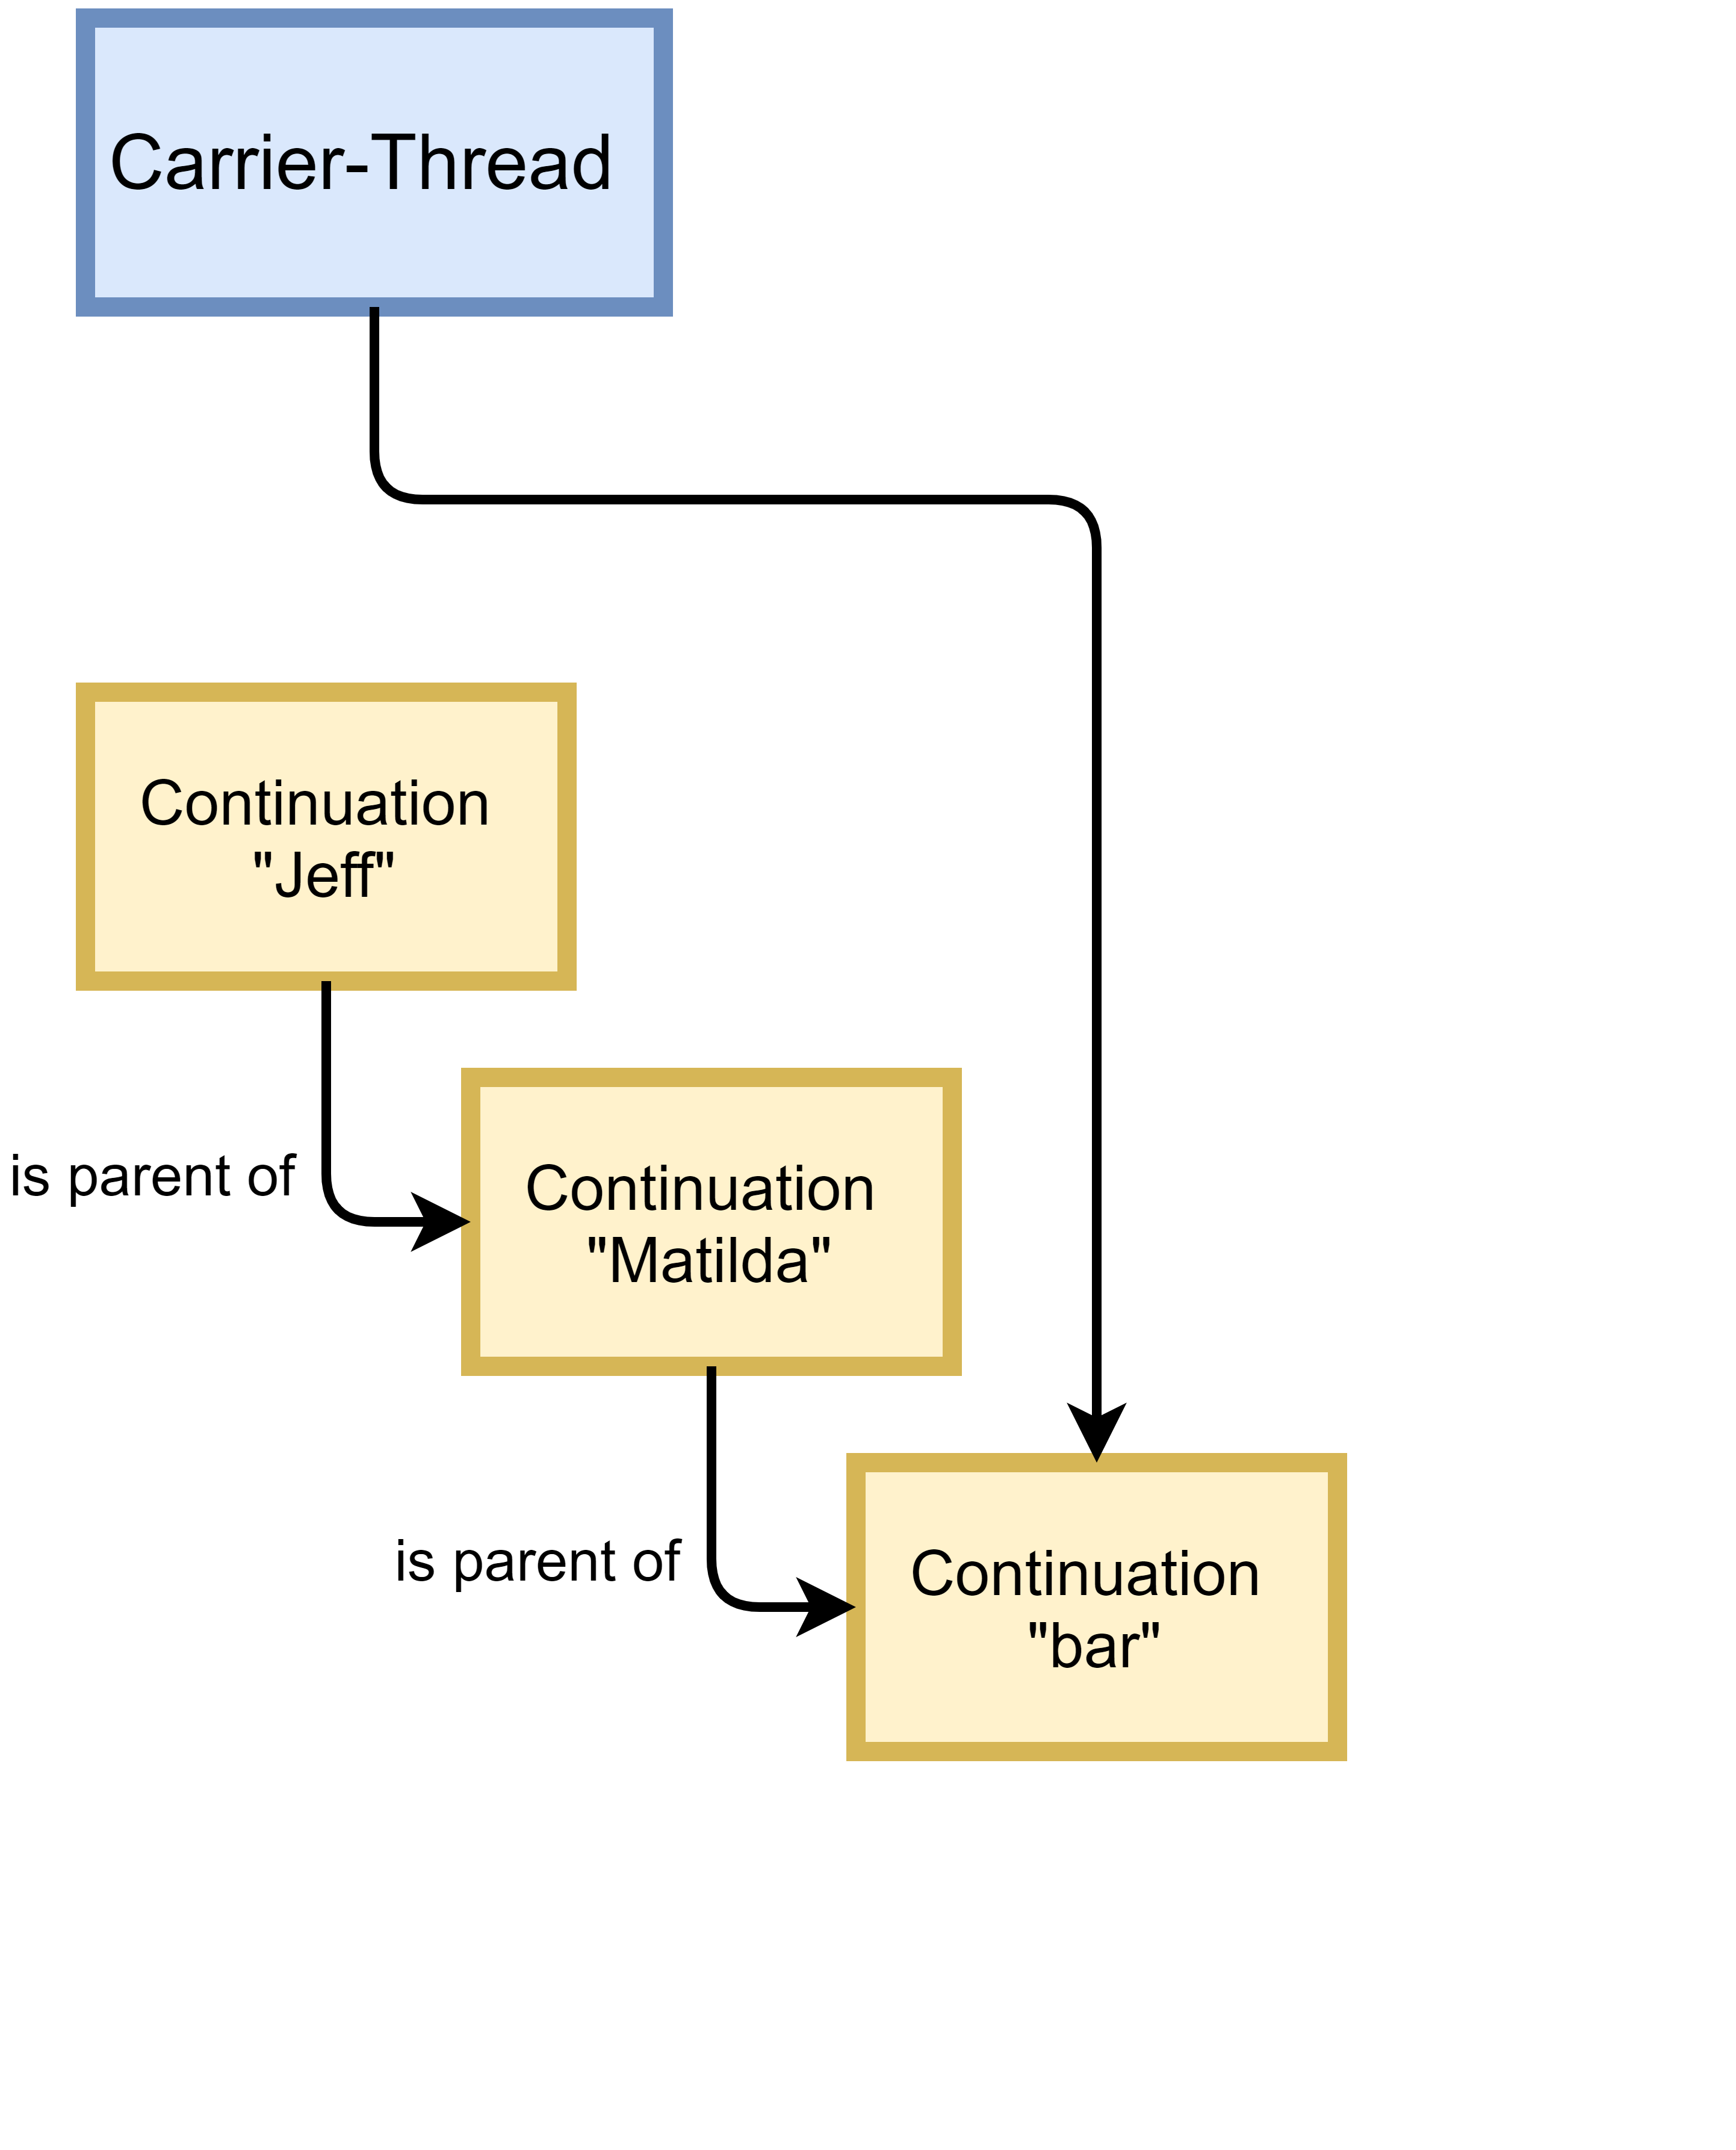
\includegraphics[width=1.0\linewidth]{img/before-run-changes-current-continuation.png}
        \label{Before Carrier-Thread's Continuation gets updated}
    \end{subfigure}
    \begin{subfigure}[b]{0.45\textwidth}
        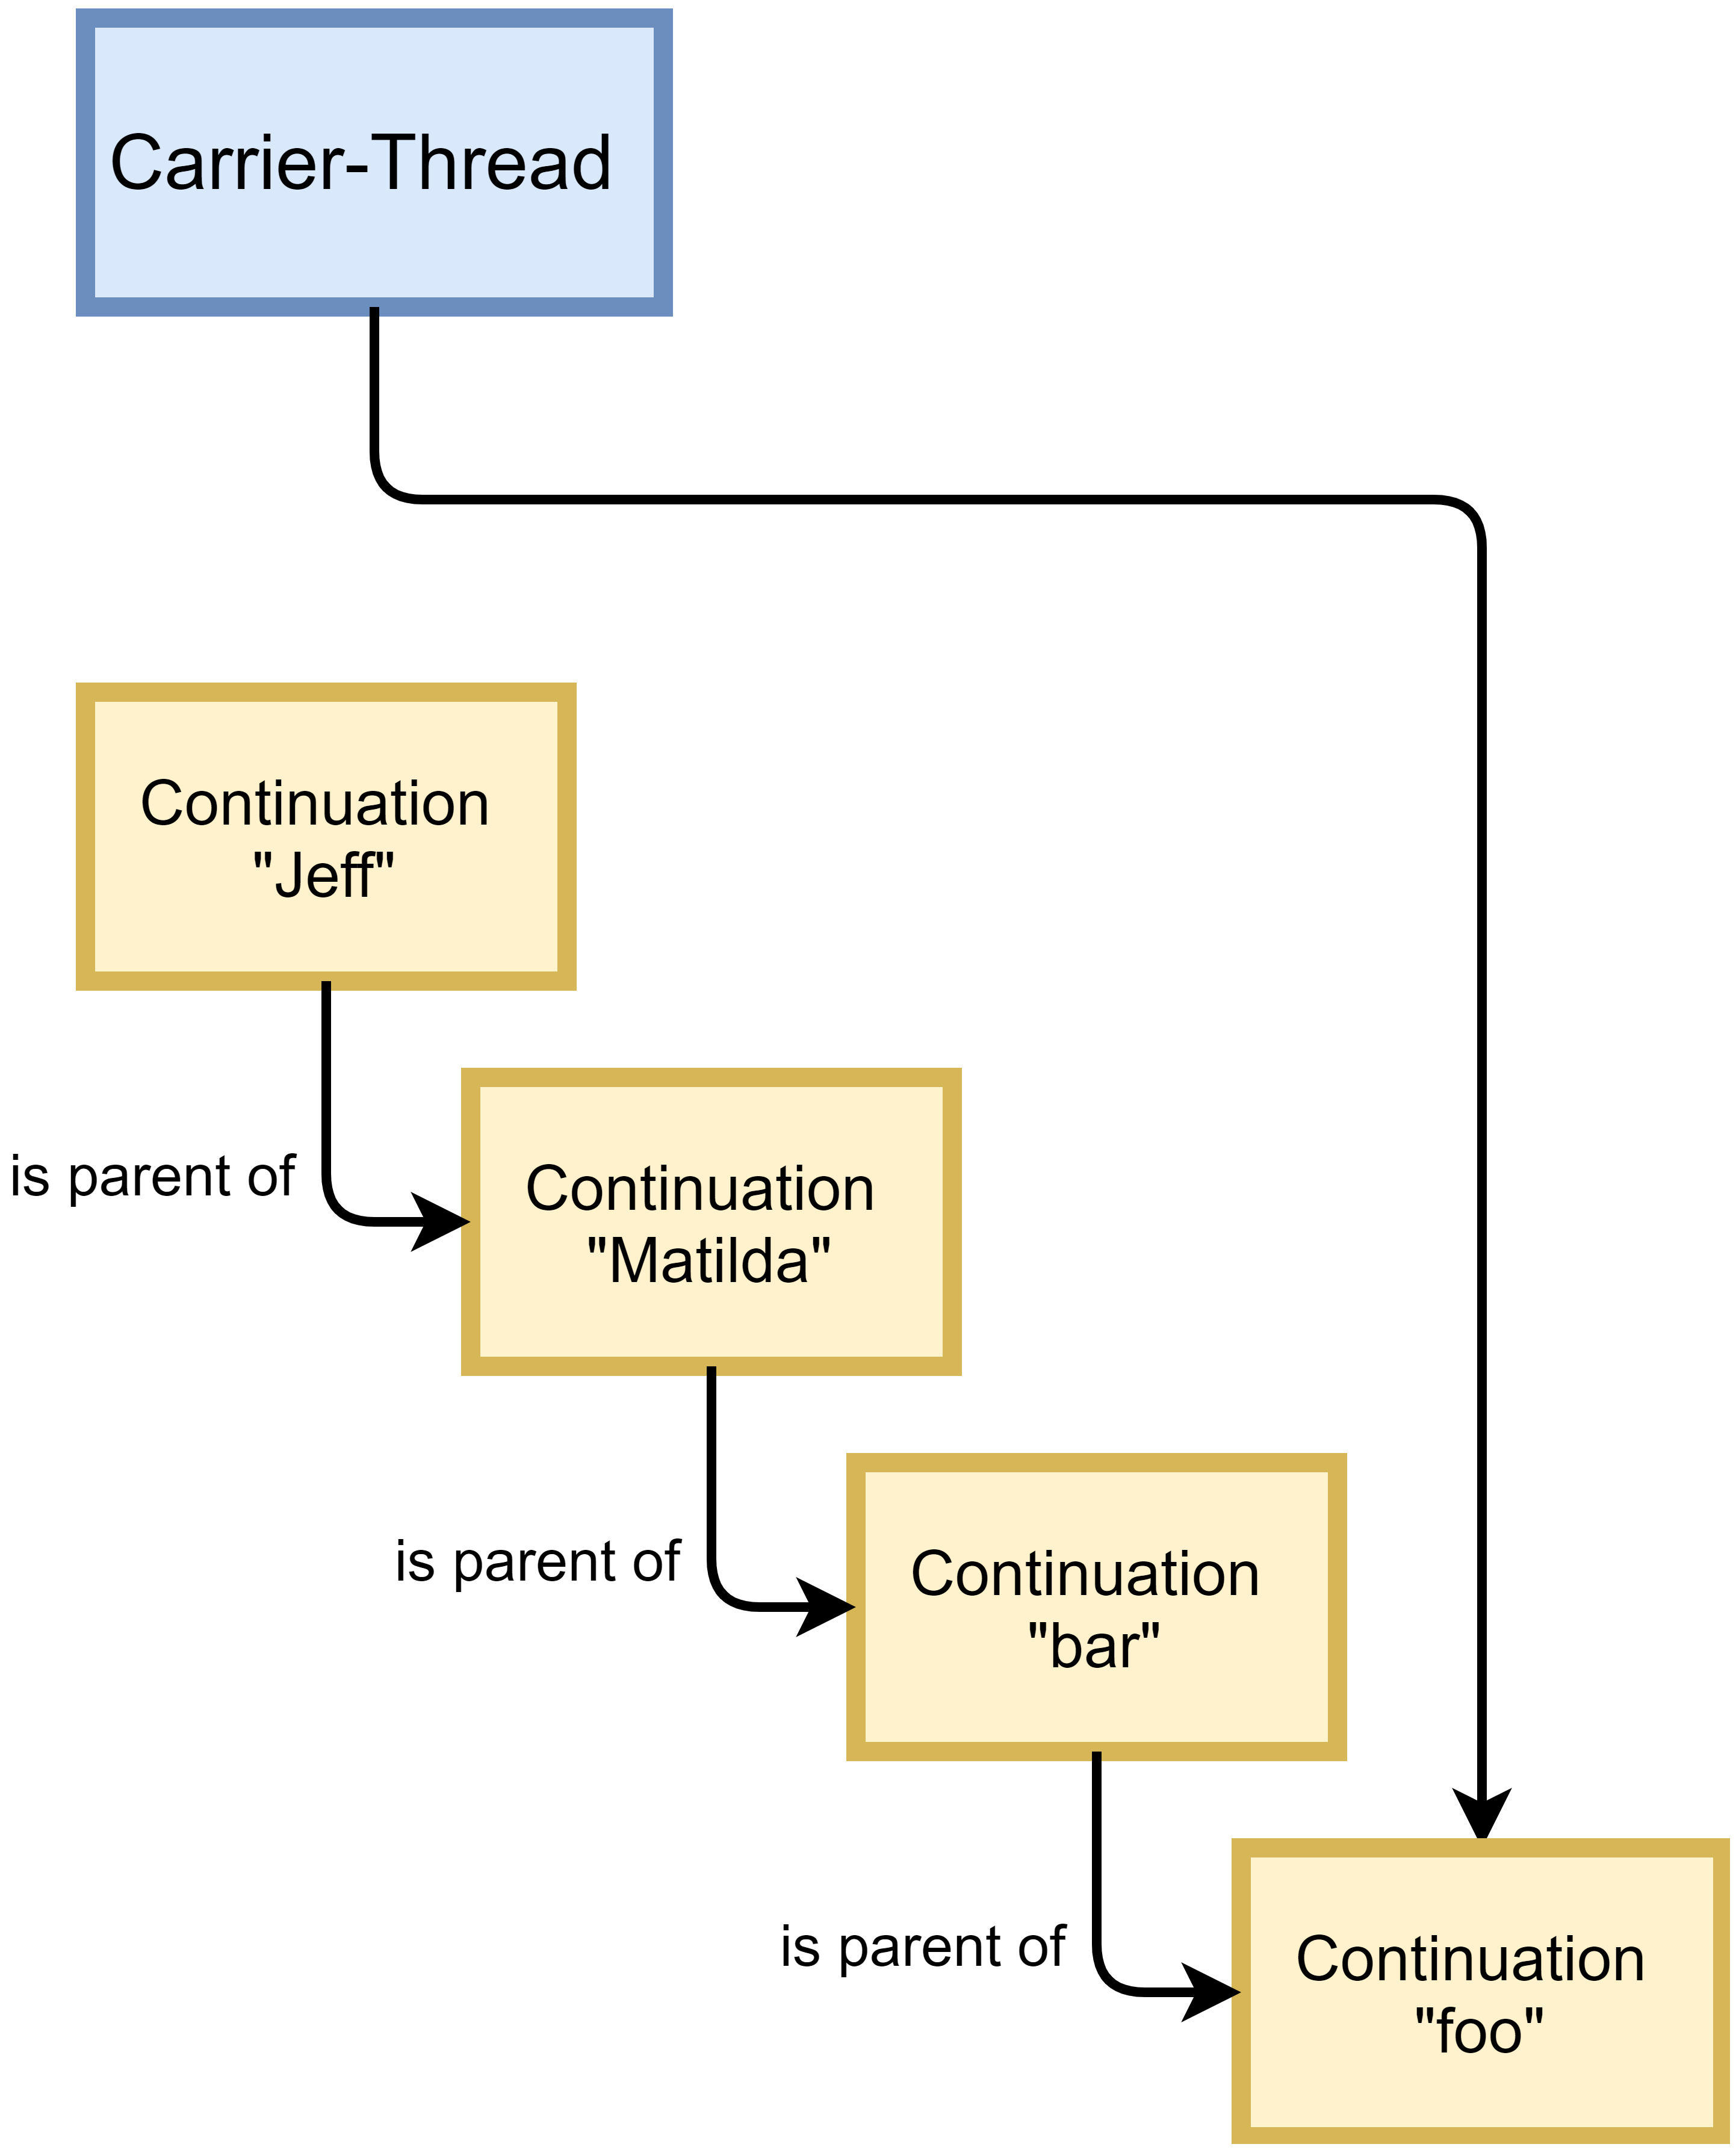
\includegraphics[width=1.0\linewidth]{img/after-run-changes-current-continuation.png}
        \label{After Carrier-Thread's Continuation gets updated}
    \end{subfigure}
    \caption{Carrier-Thread's Continuation gets updated}
\end{figure}

After that, the run method will call either the enter method or the continue method depending on whether foo is being started for the first time.
\\
\\
Once foo is done, it returns to the run method. The current carrier-thread's continuation will be set to bar. foo will be removed as a child of bar. Finally, foo will be unmounted, similar to how it was mounted at the beginning.

\subsection{Yield}
Project Loom uses three different yield functions, which are always called in the same order.
\\
First \lstinline[basicstyle=\ttfamily\color{blue}]{public static boolean yield(ContinuationScope scope)} is called. This method checks, if the current carrier-thread's continuation is part of the given ContinuationScope scope. This is done by looping a variable c through the parents of the current carrier-thread's continuation. The loop stops once c is either null or the scope of c is the same as the given scope. If c ends up being null, that means, that the program is being told to yield a ContinuationScope, while it is running a continuation, that is not part of that scope. This is undesired behavior and throws an exception. If c is not null, the program can continue and the second function will be called.
\\
\\
The other two functions are beyond the scope of this thesis, because they either are completely intrinsic or because they utilize variables that are returned from intrinsics.


\subsection{Continue}
The continue method is entirely intrinsic. Therefore it is beyond the scope of this thesis.




\section{Virtual Thread}

Similar to how threads were created as lightweight processes, virtual threads were created as lightweight threads. Therefore they line up in the hierarchy right behind the kernel threads.
\begin{figure}[H]
    \centering
    \begin{subfigure}[b]{1.0\textwidth}
        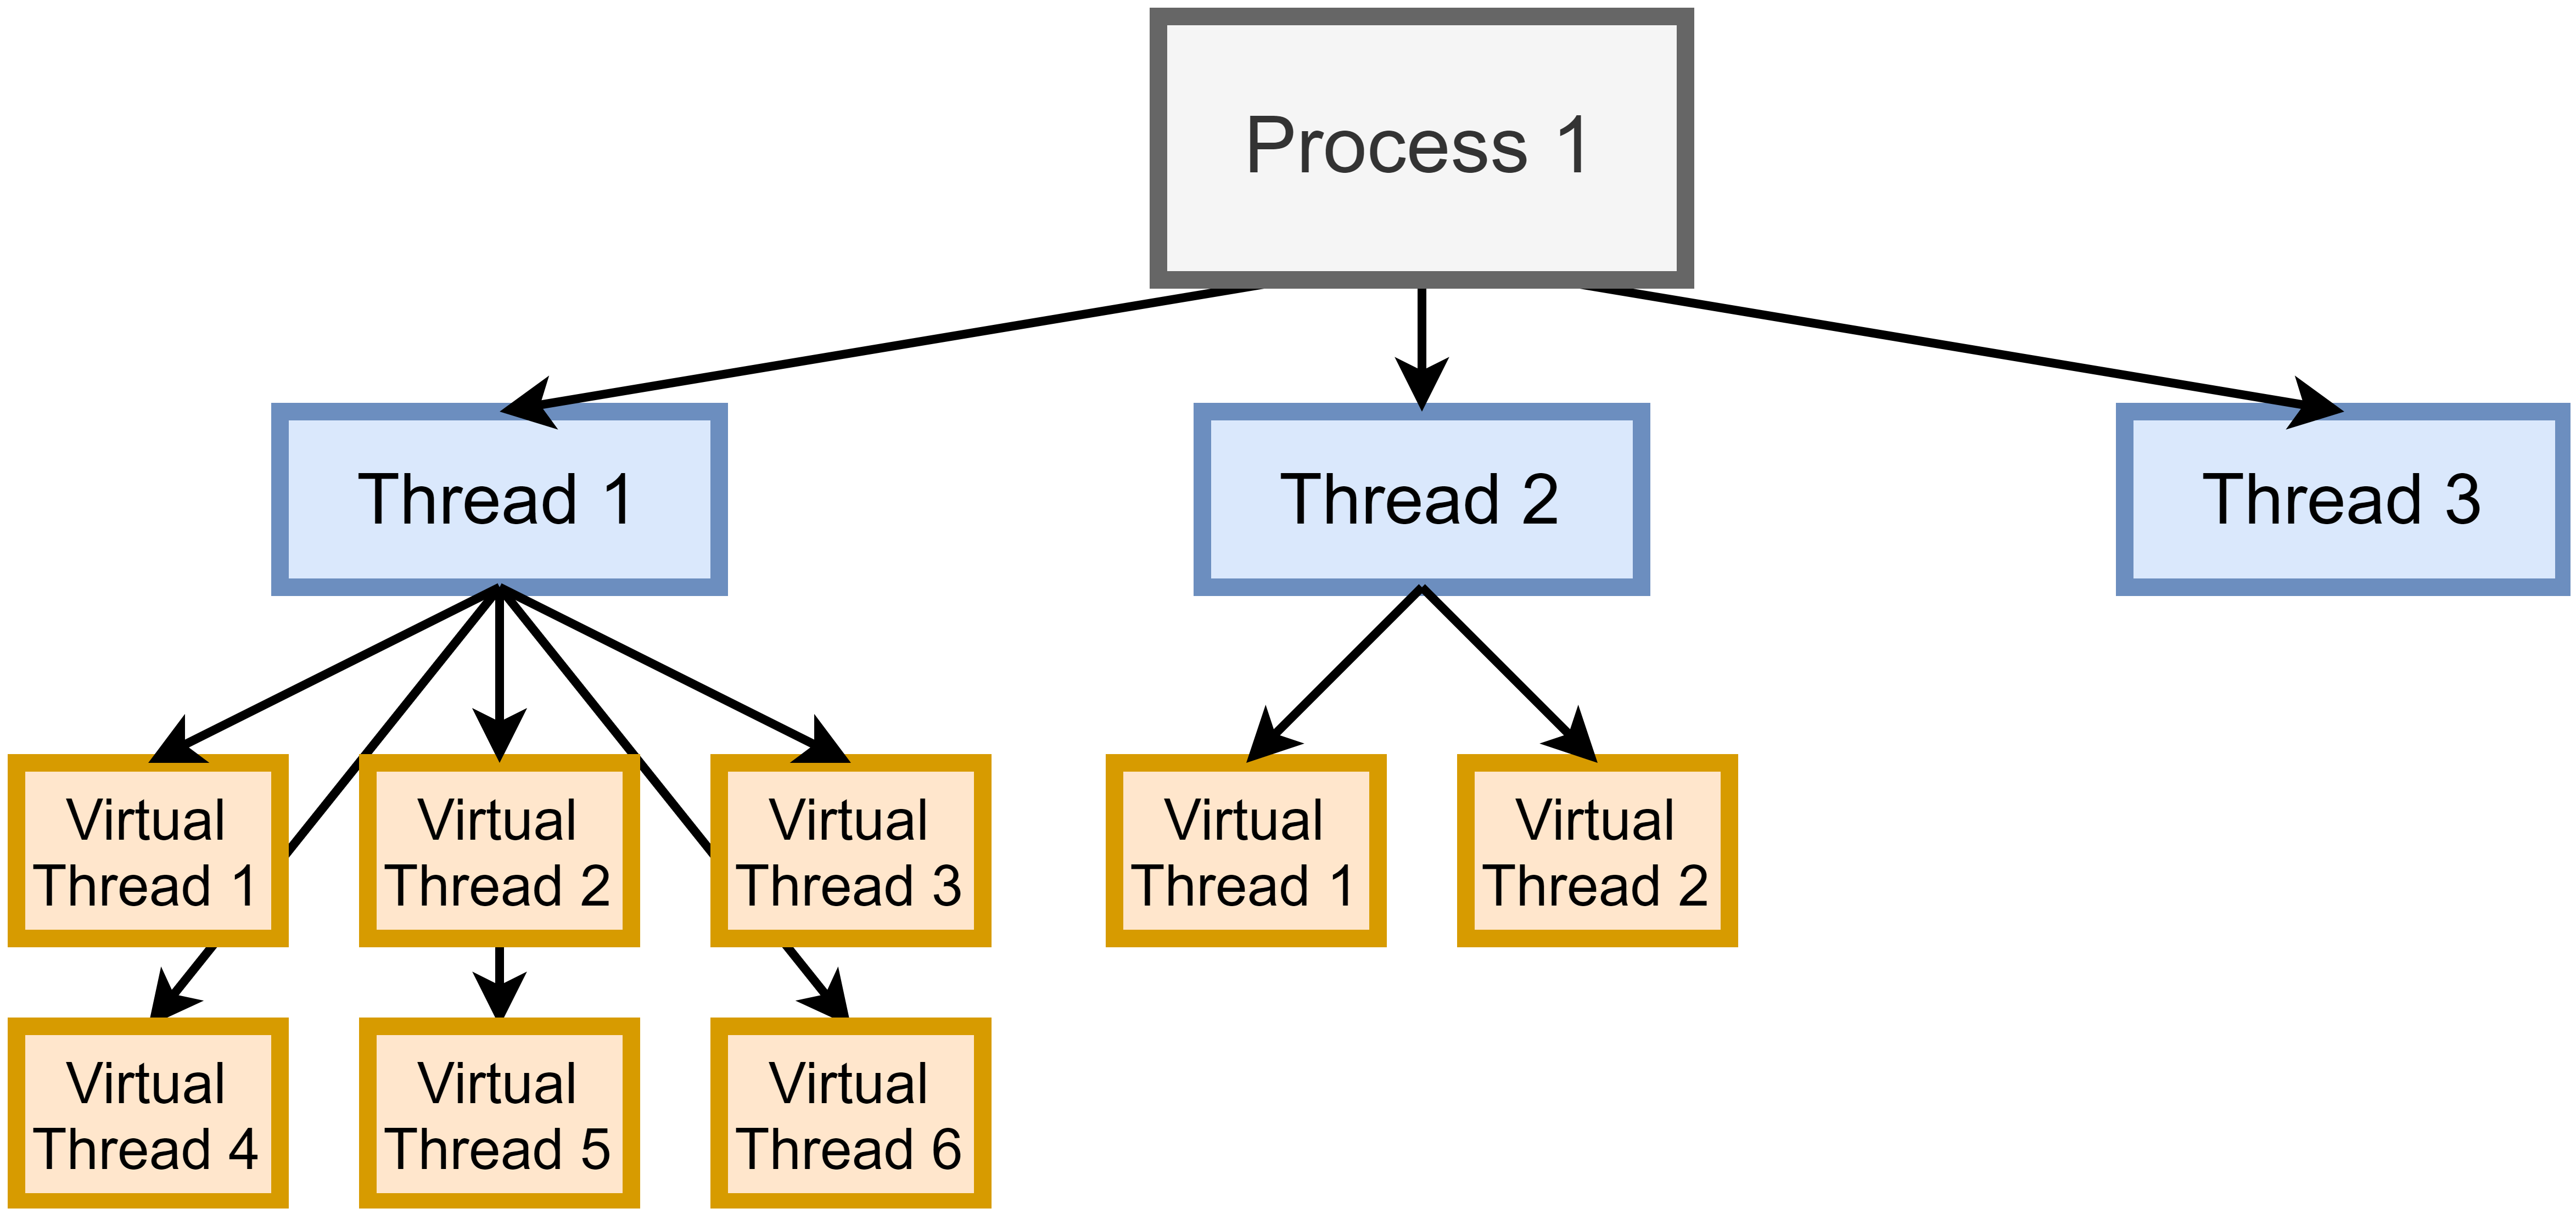
\includegraphics[width=1.0\linewidth]{img/process-thread-vthread.png}
    \end{subfigure}
    \caption{Process - Thread - Virtual Thread - Hierarchy}
    \label{Process - Thread - Virtual Thread - Hierarchy}
\end{figure}
Similar to how the scheduler of an operating system allocates CPU time to each kernel thread, the JVM allocates CPU time to each virtual thread. The scheduler is not the focus of this work. It will be briefly addressed in the next chapter.
\begin{figure}[H]
    \centering
    \begin{subfigure}[b]{1.0\textwidth}
        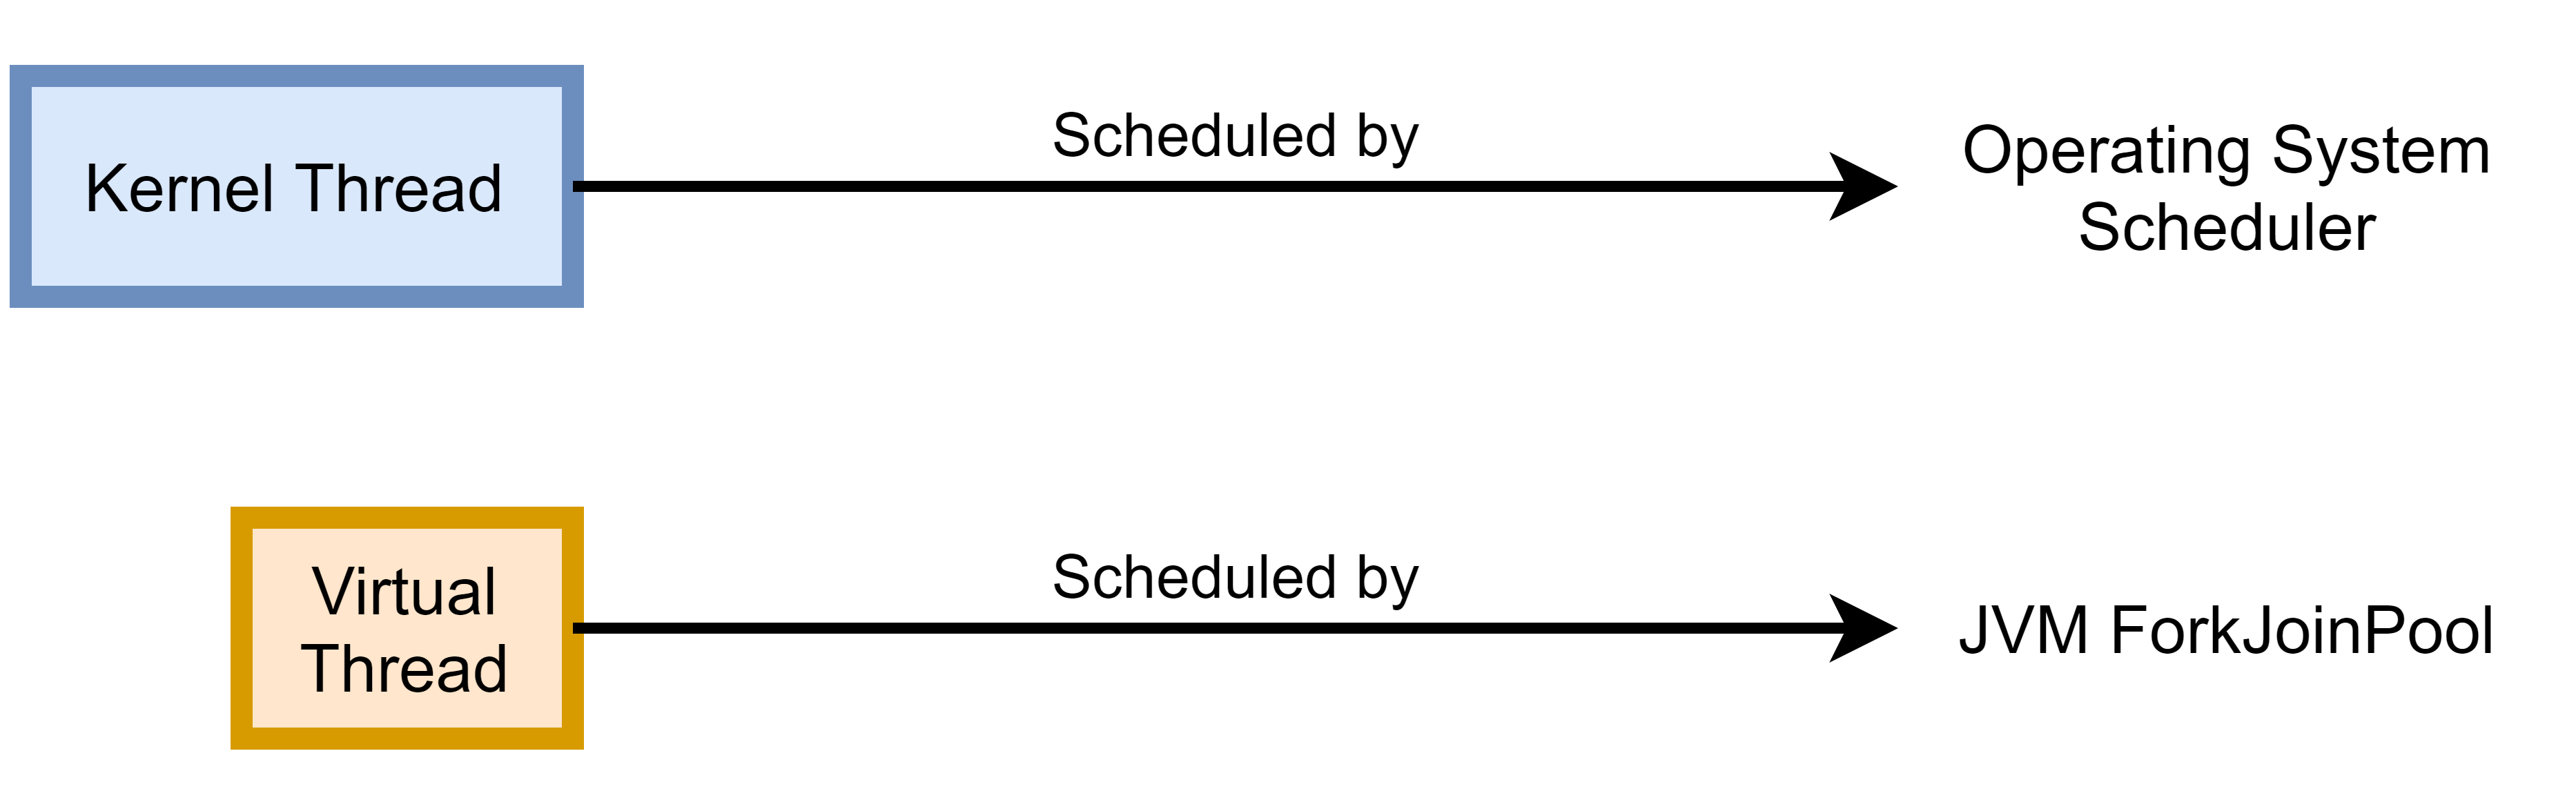
\includegraphics[width=1.0\linewidth]{img/thread-vthread-scheduler.png}
    \end{subfigure}
    \caption{Thread - Virtual Thread - Scheduler}
    \label{Thread - Virtual Thread - Scheduler}
\end{figure}
The virtual thread class is a high level class. Underneath it the low level continuation class is at work. Direct interaction with the continuation class is currently possible, but developers are advised to use virtual threads instead. QUOTE: Continuations will probably move to a non-exported package at some point (stand in einer email, wahrscheinlich direkt an ihn selbst addressiert gewesen, wie zitieren?)




\subsection{Examples}

\myparagraph{Virtual Thread vs Kernel Thread}
The following code excerpt shows very well, how simple the transition from kernel to virtual threads is envisioned to be by project Loom.

\begin{lstlisting}[language=custom-java]
    Runnable printThread = () -> System.out.println(Thread.currentThread());

    var virtualThreadFactory = Thread.builder().virtual().factory();
    var kernelThreadFactory = Thread.builder().factory();

    var virtualThread = virtualThreadFactory.newThread(printThread);
    var kernelThread = kernelThreadFactory.newThread(printThread);

    virtualThread.start();
    kernelThread.start();
\end{lstlisting}
The code above first creates a Runnable called printThread.
Then a ThreadFactory is created for both kernel and virtual threads.
These ThreadFactories are used to create a virtual and a kernel thread.
Afterwards, both threads are started. \cite{Baeldung:Threads}

\subsection{Structured Concurrency}
The ExecutorService class can be used to bring structured concurrency to virtual threads.
\\
\\
Here, the program will only continue once both tasks inside the try-block are finished.

\begin{lstlisting}[language=custom-java,caption={Structured Concurrency - Simple \cite{loom:structured-concurrency}},captionpos=b]
    ThreadFactory factory = Thread.builder().virtual().factory()

    try (ExecutorService executor = Executors.newUnboundedExecutor(factory)) {
        executor.submit(task1);
        executor.submit(task2);
    }
\end{lstlisting}

Here, the main program will only continue once foo and bar are done. Similar to that foo and bar are only going to be done, once the methods inside their try-blocks are done.
\begin{lstlisting}[language=custom-java,caption={Structured Concurrency - Nested \cite{loom:structured-concurrency}},captionpos=b]
    ThreadFactory factory = Thread.builder().virtual().factory()

    try (ExecutorService executor = Executors.newUnboundedExecutor(factory)) {
        executor.submit(() -> foo());
        executor.submit(() -> bar());
    }

    void foo() {
        try (ExecutorService executor = Executors.newUnboundedExecutor(factory)) {
            executor.submit(...);
        }
    }

    void bar() {
        try (ExecutorService executor = Executors.newUnboundedExecutor(factory)) {
            executor.submit(...);
        }
    }
\end{lstlisting}

This example works very similar to the first one. The only change is, that a deadline of 30 seconds has been added. Once the deadline is hit, all tasks inside the try block are going to be canceled. If those tasks started additional tasks inside themselves, those tasks will also be canceled.

\begin{lstlisting}[language=custom-java,caption={Structured Concurrency - Deadlines \cite{loom:structured-concurrency}},captionpos=b]
    ThreadFactory factory = Thread.builder().virtual().factory()
    var deadline = Instant.now().plusSeconds(30);

    try (ExecutorService executor = Executors.newUnboundedExector(factory).withDeadline(deadline)) {
        executor.submit(task1);
        executor.submit(task2);
    }
\end{lstlisting}


\section{ForkJoinPool}
Per default virtual threads use the Java ForkJoinPool as their scheduler. Project Loom considers this scheduler to be "excellent" \cite{loom:proposal}. Knowledge regarding the ForkJoinPool is not necessary to work with virtual threads. The creation and maintenance of the scheduler is part of the virtual thread class. However, if a developer wants to use their own scheduler, it is easily possible:

\begin{lstlisting}[language=custom-java]
    CustomScheduler scheduler = new CustomScheduler();
    ThreadFactory factory = Thread.builder().virtual(scheduler).factory();
\end{lstlisting}

The developer creates an instance of their custom scheduler and passes it as an argument when creating the ThreadFactory.















